\documentclass[12pt]{article}
\usepackage[latin1]{inputenc} 
\usepackage{amsmath,amsfonts,amssymb,amsthm}
\usepackage[auth-sc,affil-sl]{authblk}
\usepackage[spanish]{babel}
\usepackage{graphicx}
\usepackage{natbib}

% 
\setlength{\parindent}{0pt}
\setlength{\textwidth}{6.3in}
\setlength{\topmargin}{-33pt}
\setlength{\oddsidemargin}{0pt}
\setlength{\evensidemargin}{0pt}
\setlength{\textheight}{8in}


% cosas del authblk
\setlength{\affilsep}{1mm}
\renewcommand\Authfont{\small} %\scshape\normalsize
\renewcommand\Affilfont{\itshape\small}

\renewcommand\Authsep{  }
\renewcommand\Authand{ }
\renewcommand\Authands{ }


% definiciones
\newcommand{\keywordname}{Palabras clave}
\newenvironment{keywords}{%
    \paragraph*{\keywordname: }}%
    {}{}
\newcommand{\area}{{\bf Area:} {\sc M\'etodos Cuantitativos.}}%{\small}


%********************************************%********************************************%********************************************

\begin{document}

\thispagestyle{empty} 
\begin {center}


UNIVERSIDAD DE LA REP�BLICA

Facultad de Ciencias Econ�micas y de Administraci�n

Licenciatura en Estad�stica

\vspace{4.5 cm}


\textbf{\large  T�tulo del trabajo}


\vspace{1.5 cm}

\textbf{Fulana, Mengano}\\
\textbf{Noviembre 2017}


\end{center}


\vspace{3.5cm}

\begin{center}
\textbf{Trabajo final de Taller de Simulaci�n Monte Carlo}\\
\vspace{1.0 cm}

\end{center}

\newpage

\setcounter{page}{1} 

\begin{center}
\textbf{ T�tulo del trabajo}
\end{center}
\begin{center}
Fulana \footnote{fulana@xxxx.xxx.uy}\\
{\small\emph{Licenciatura en Estad�stica}}
\end{center}
 
 
\begin{center}
Mengano \footnote{mengano@xxx.xxx.uy}\\
{\small\emph{Licenciatura en Estad�stica}}
\end{center}

\begin{center}
\textbf{RESUMEN}
\end{center}

Bla, Bla, Bla



\textbf{Palabras claves}: an\'alisis del error, bondad de ajuste, integraci�n, m\'etodos.

\pagebreak

\section{Introducci�n}

En este documento se presenta .....

\section{Planteo del problema}
\label{sec:modelo}


\begin{center}
\begin{equation} \label{eq:bernoulli}
	P(X=x)=p^{x}(1-p)^{1-x}
\end{equation}
\end{center}



\section{Metodolog�a}



\begin{table}[htbp]
	\centering
		\begin{tabular}{ccc}
			\hline
			par\'ametro	&	estimaci�n	&	error est\'andar	\\
			\hline
			Datos Completos & & \\
			\hline
			\quad $\widehat{\phi}_1$	&	0,358	&	0,033	\\
			\quad $\widehat{\phi}_2$	&	1,488	&	0,141	\\
			\quad $\widehat{\alpha}_{12}$	&	2,291	&	0,223	\\
			\hline
			Datos Incompletos & & \\
			\hline
			\quad	$\widehat{\phi}_1$	&	0,226	&	0,022	\\
			\quad	$\widehat{\phi}_2$	&	1,362	&	0,129	\\
			\quad	$\widehat{\alpha}_{12}$	&	3,509	&	0,356	\\
			\hline
		\end{tabular}
	\caption{Estimaciones sobre datos completos e incompletos}
	\label{tab:est1}
\end{table}
\pagebreak
\section{Aplicaci�n}
\label{sec:apli}

para poner salida de la consola de R

\begin{verbatim}
  nrounico Depart sexo edad   salud univ sang1617   sang11 sang2627   sang31
1        2    PAY    M   40 privada   SI     sano     sano     sano     sano
2        5    PAY    M   21 privada   NO     sano     sano     sano     sano
4       10    PAY    M   21 publica   SI     sano     sano presente presente
5       11    PAY    F   66 publica   NO presente presente presente presente
 sang3637 sang4647 tramo_eta_rec inse sext1 sext2 sext3 sext4 sext5 sext6
1     sano     sano    de 35 a 44   41     0     0     0     0     0     0
2     sano     sano    de 15 a 24   36     0     0     0     0     0     0
4     sano     sano    de 15 a 24   62     0     0     1     0     1     0
5 presente presente    de 65 a 74   19     1     1     1     1     1     1
\end{verbatim}

\begin{figure}
	\centering
	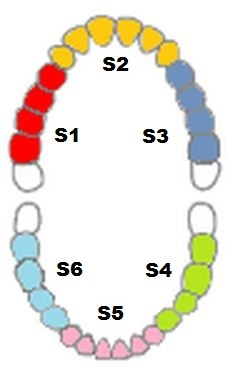
\includegraphics[width=0.30\textwidth]{sextantes.JPG}
	\label{fig:sextantes}
	\caption{Distribuci�n de los sextantes en la boca}
\end{figure}

Tabla
 
\begin{table}[htbp]
	\centering
		\begin{tabular}{cccc}
				\hline
			    	&	presencia	&	ausencia	&	\%	\\
				\hline							
				S1	&	195	&	1288	&	13,1	\\
				S2	&	171	&	1312	&	11,5	\\
				S3	&	209	&	1274	&	14,1	\\
				S4	&	223	&	1260	&	15,0	\\
				S5	&	364	&	1119	&	24,5	\\
				S6	&	211	&	1272	&	14,2	\\
				\hline							
		\end{tabular}
	\caption{Presencia de sangrado por sextantes}
	\label{tab:sang1}
\end{table}

\begin{center}
\begin{footnotesize}

\begin{verbatim}
> int.conf(modelo1,0.05)
---------------------------------------------------- 
intervalos de confianza al 95% para las intensidades 
---------------------------------------------------- 
                  int.inf   int   int.sup
               1   0.031   0.042   0.054
               2   0.023   0.033   0.043
               3   0.031   0.043   0.055
               4   0.022   0.032   0.042
               5   0.113   0.137   0.161
               6   0.033   0.045   0.057
---------------------------------------------------- 
intervalos de confianza al 95% para las asociaciones 
---------------------------------------------------- 
                     asoc.inf  asoc    asoc.sup
               1-2    2.151    4.010    5.868
               1-3    4.338    7.392   10.446
               1-4    0.845    1.780    2.714
               1-5    0.899    1.651    2.402
               1-6    0.807    1.643    2.478
               2-3    1.222    2.298    3.374
               2-4    0.542    1.161    1.781
               2-5    2.161    3.872    5.583
               2-6    1.160    2.307    3.455
               3-4    1.376    2.700    4.024
               3-5    1.193    2.085    2.978
               3-6    1.050    2.035    3.020
               4-5    3.642    6.256    8.870
               4-6    5.376    8.978   12.580
               5-6    1.124    1.951    2.777
\end{verbatim}
\end{footnotesize}

\end{center}
%\pagebreak
\subsection{Discusi�n}
\label{sec:Discu}
Puede verse en este caso que ...
 
Vi\~neta 
\begin{enumerate}
\item Se descarta la hip�tesis de que la presencia de sangrado es independiente entre algunos  sextantes.\\
\item Se constata que la asociaci�n de presencia de sangrado entre los sextantes posteriores no difiere entre mand�bula y maxilar.\\
\end{enumerate}

\section{Conclusiones y comentarios finales}

\nocite{Alvarez2012}
\pagebreak 
\begin{appendix}
\section{Ap\'endice}

Ac\'a van los scripts usados para los c\'alculos
\end{appendix}

\bibliographystyle{apalike}
%\bibliographystyle{econometrica}
\bibliography{biblioBer}

\end{document}
